%!TEX root = ../assignment1.tex

\section{Findings Of Phase 2}

\subsection{Overview Of Data}
In Phase 2, 10 case studies are given on how projects failed in Victoria Australia. The cases are government related information communication and technology projects. The author\parencite{case_study} provides well structured anatomy of projects where issues are discussed in depth by topics. Additionally, some recommendations are given by the author, some of which are responded by the project owners.

\subsection{Gaps and Solutions}
Using the same method, we collect gaps and possible solutions(proposals) for further evaluation. There are 54 sections of gaps reflecting 54 proposals to 10 case studies. The author uses no mathematical model to prioritize gaps, a baseline value of $1$ is also used to all the proposals, according to the predefined methodology.

The collected data are tagged with the same four themes: control, process, people and structure. Here are some samples under each theme.

\subsubsection{Samples: Control}
% id 21
In case 4, the author argues that the longer planning that spans in time, the more risk of redesigned. Ultimately, project will be likely to fail due to this uncertainty of change. In initial phase of project, project leaders should plan funding well in initial phase with top management support.
\begin{quotation}
The longer it takes to fund the project, the longer it will take for the outdated systems to be replaced, the more likely it is the costs will be increased and the more likely it is that the project will need to be redesigned.
\end{quotation}


% id 2
In case 1, it is the rushing to meet deadlines that fails to deliver design goals. For cover-up, benefits are altered to please government. Project managers should define measurement of deliverables and change accordingly. 
\begin{quotation}
The business case was rushed to meet budget timelines and to fit within the funding already allocated by the government. It failed to identify measurable benefits. Instead, benefits were written to obtain government support.
\end{quotation}

\subsubsection{Samples: Process}
% id 26
poor user training and post-implementation support result in bad experience among users. Better user training and support should be designed and implemented in early stage of project planning.

\begin{quotation}
Despite being introduced in July 2008, CRIS continues to suffer from inadequate training, poor help-desk support, and slow responses to functionality change requests.
\end{quotation}

% 30
training cost is not included in the planning process. It is suggested to consider training in cost planning.
\begin{quotation}
Training costs have not been fully calculated or recorded against the project. The original business case indicated training would  cost \$23 million.
\end{quotation}

\subsubsection{Samples: People}
% 34
failing to detect risk of vendor results in bad contract deals. Vendor support should be reviewed by a third party in planning.
\begin{quotation}
A change in vendor ownership and concerns of vendor withdrawal led to DOJ making contractual concessions.
\end{quotation}

% 37
project fails and leads to alternative solution when requirements are not communicated precisely. It is import to understand requirements and define deliverables between project manager and users.
\begin{quotation}
According to the Supreme Court, ICMS’s case management system (CourtView) fails to meet the court’s needs. The Supreme Court has ultimately resolved to pilot its own system to provide case management.
\end{quotation}

\subsubsection{Samples: Structure}
% 4
The vacancy of a project leader results management chaos. It is important to have a project leader.
\begin{quotation}
Victoria Police failed to appoint a single, qualified project manager to run the project, notwithstanding that project management was identified as a project risk in the business case and a major contributor to the failure of 60-70 per cent of ICT-related projects.
\end{quotation}

% 19
The organization structure stops from making a timely funding to implement the project. A better organization is advised.
\begin{quotation}
The government approved VicRoads spending \$52 million on RandL over three years while the Cabinet budget committee was apparently uncertain about the project and there was a risk that the project would not receive the required funding. This risk eventuated.
\end{quotation}
\subsection{Evaluation Of Solutions}
To select the solutions out of all the proposals, we do the same evaluation steps as shown in \ref{section:evaluation}.

With the defined method, we tag all our research contexts as $C_{1}, C_{2}, \ldots, C_{10}$. We assume all the solutions from the 10 case studies are of equal importance, given the fact that there is no math model used in Phase 2. Therefore, we pad the cross-contextual coefficient with a baseline value of 1 to all the $\mathit{k_{C_{i},j}}$ in formula \ref{brief}. So formula \ref{final} can be simplified as 

\begin{equation}
g_{C_{i},j} = l_{C_{i},j} = |P_{C_{i,j}}| |R_{C_{i,j}}|
\label{formula:p2}
\end{equation}

With the updated formula \ref{formula:p2}, we calculate the global influence score for each proposal. Here is a visualization of the scores of all the proposals in Phase 2.

In the plot, there are 3 groups: the leading group of 3 proposals, the group of majority and the trailing group.

\begin{figure}[ht]
\centering
\resizebox{\columnwidth}{!}{%
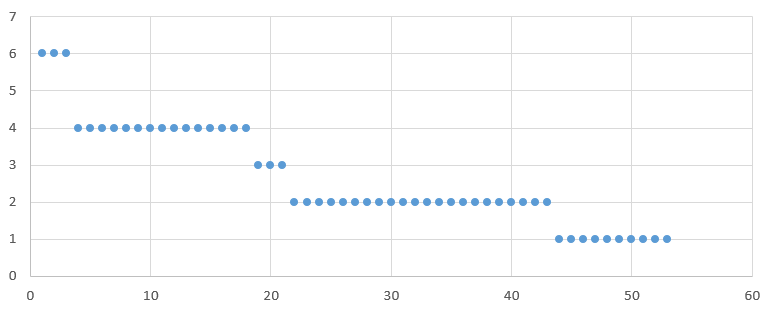
\includegraphics{global_influence_score_p2.png}
}
\end{figure}
\subsection{Result Of Evaluation}
We calculate the average score using the same way($\bar{g}=1.37$), which truncates the trailing group. The selected proposals are shown as follows.

\begin{table}[ht]
\caption{Solution List Of Phase 2}
\resizebox{\columnwidth}{!}{%
\csvautotabular{tables/solutions_p2.csv}
}
\label{tab:solution2}
\end{table}